\documentclass[border=5mm]{standalone}
\usepackage{tikz}
\begin{document}
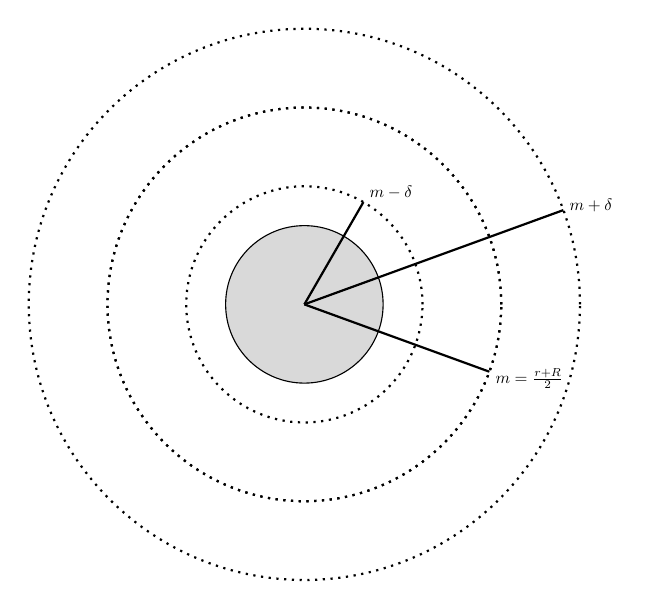
\begin{tikzpicture}[
  every node/.style={scale=0.6}
]
% inner/outer circle:
\filldraw [fill=gray!30, draw=black] (0,0) circle[radius=1];


%\fill before \draw... repeat loop! (sigh)
\foreach \radius in {2.5,3.5} {
  \draw [even odd rule, black, thick, dotted] (0,0) circle[radius=(\radius-1)] circle[radius=\radius];
}
  \draw [thick] (0,0) -- (60:1.5cm) node[anchor=200] {$m-\delta$};
  \draw [thick] (0,0) -- (20:3.5cm) node[anchor=190] {$m+\delta$};
  \draw [thick] (0,0) -- (-20:2.5cm) node[anchor=170] {$m=\frac{r+R}{2}$};

\end{tikzpicture}
\end{document}